
\documentclass[final,leqno]{siamltex704}
%\documentclass[leqno]{siamltex704}
\usepackage{epsfig}
\usepackage{amsmath,bm}
\usepackage{amssymb}
\usepackage{float}
\usepackage{tikz}
\usepackage{graphicx}
\usepackage[notcite,notref]{showkeys}
\newtheorem{algorithm}{Weak Galerkin Algorithm}
\newcommand{\bq}{{\bf q}}
\newcommand{\bn}{{\bf n}}
\newcommand{\bx}{{\bf x}}
\newcommand{\bv}{{\bf v}}
\def\bbb{{\bf b}}
\def\T{{\mathcal T}}
\def\E{{\mathcal E}}
\def\V{{\mathcal V}}
\def\W{{\mathcal W}}
\def\F{{\mathcal F}}
\def\l{{\langle}}
\def\r{{\rangle}}
\def\jump#1{{[\![#1[\!]}}
\def\bbF{{\bf F}}
\def\bbf{{\bf f}}
\def\bn{{\bf n}}
\def\bq{{\bf q}}
\def\bV{{\bf V}}
\def\bu{{\bf u}}
\def\bv{{\bf v}}
\def\bw{{\bf w}}
\def\br{{\bf r}}
\def\bs{{\bf s}}
\def\bbQ{\mathbb{Q}}
\def\bfQ{\bf{Q}}
\def\bcurl{ \textbf{curl }}
\def\bE{{\bf E}}
\def\bB{{\bf B}}
\def\bx{{\bf x}}
\def\bU{{\bf U}}
\def\bV{{\bf V}}
\def\bJ{{\bf J}}
\def\be{{\bf e}}
\def\mL{{\mathcal L}}
\def\mF{\mathcal{F}}

\def\ljump{{[\![}}
\def\rjump{{]\!]}}

\def\lavg{{\{\!\{}}
\def\ravg{{\}\!\}}}

\def\aa{\mathfrak{a}}
\def\bbQ{\mathbb{Q}}
\newcommand{\pT}{{\partial T}}
\newtheorem{defi}{Definition}[section]
\def\3bar{{|\hspace{-.02in}|\hspace{-.02in}|}}
%\setlength{\textwidth}{6truein} \setlength{\textheight}{8truein}
%\voffset=-0.55truein
%\hoffset=-0.65truein
\renewcommand{\ldots}{\dotsc}
\setlength{\parskip}{1\parskip}

\title{Discontinuous Galerkin Sparse Grids Methods for Helmholtz Equations}


\author{
}

\begin{document}

\maketitle

\begin{abstract}
\end{abstract}

\begin{keywords}
Helmholtz equations, discontinuous Galerkin method, sparse grids methods.
\end{keywords}

\begin{AMS}
Primary: 65N15, 65N30; Secondary: 35J50
\end{AMS}
\pagestyle{myheadings}

\section{Introduction}
The Helmholtz equation is the simplest possible model of wave propagation. Although most applications are concerned with the propagation of waves in exterior domains, it is common to use as a model problem the Helmholtz equation posed in an interior domain with an impedance boundary conditions, i.e.,
\begin{eqnarray}
\Delta u+k^2 u &=& -f \mbox{ in }\Omega,\\
\frac{\partial u}{\partial \bf n}-\text{i}ku &=& g,\mbox{ on }\Gamma.
\end{eqnarray}

We shall consider about the discretization of the original Helmholtz problem with a complex shift
\begin{eqnarray}
\Delta u+(k^2+\text{i}\epsilon) u &=& -f \mbox{ in }\Omega,\\
\frac{\partial u}{\partial \bf n}-\text{i}\eta u &=& g,\mbox{ on }\Gamma.
\end{eqnarray}

The following DG scheme will be utilized in the computing: find $u\in V_h$, such that
\begin{eqnarray}
A_{\epsilon}(u_h,v) = (f,v)+\langle g,v \rangle_{\Gamma},\ \forall v\in V_h,
\end{eqnarray}
where
\begin{eqnarray*}
A_{\epsilon}(u_h,v)&=&(\nabla_h u_h,\nabla_h v)-(k^2+\text{i}\epsilon)(u,v)-\langle\lavg\nabla u_h\ravg,\ljump v\rjump\rangle_{\mathcal{E}_h^0}-\langle\lavg\nabla v\ravg,\ljump u_h\rjump\rangle_{\mathcal{E}_h^0}\\
%%%%%%
&+&\frac{\alpha}{h}\langle\ljump u_h\rjump,\ljump v\rjump\rangle_{\mathcal{E}_h^0}-\langle\text{i}\eta u,v\rangle_{\Gamma}.
\end{eqnarray*}
The original Helmholtz equation that we are interested in solving, is taking $\epsilon = 0$ and $\eta = k$, and in this case we write $A(u,v)$ instead of $A_{\epsilon}(u,v)$.

The Galerkin equation are equivalent to the linear system
\begin{eqnarray}
\mathbb{A}_{\epsilon}{\bf u}={\bf f}.
\end{eqnarray}

% results from REF
\begin{figure}[H]
\centering
\begin{tabular}{ccc}
  {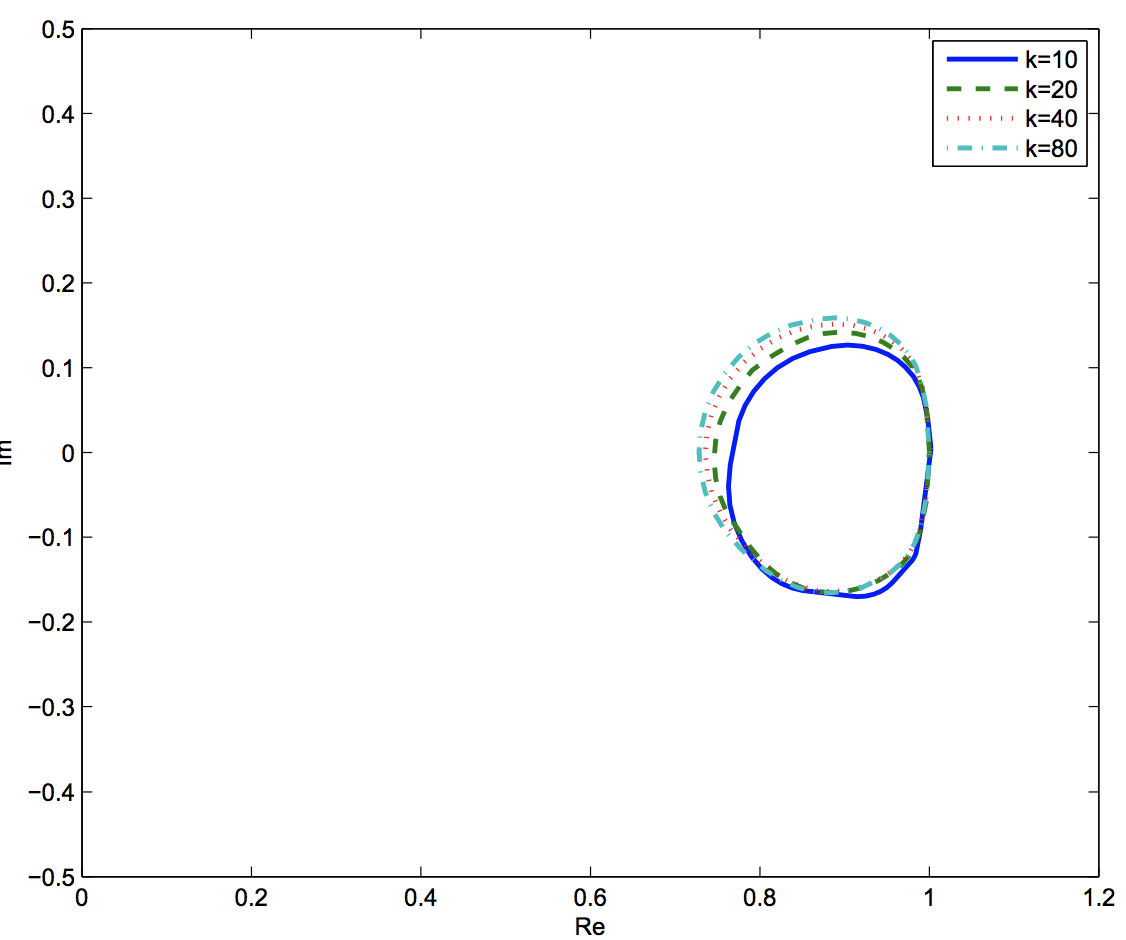
\includegraphics[width=.31\textwidth]{./Ref-fig/epsk}}&
  {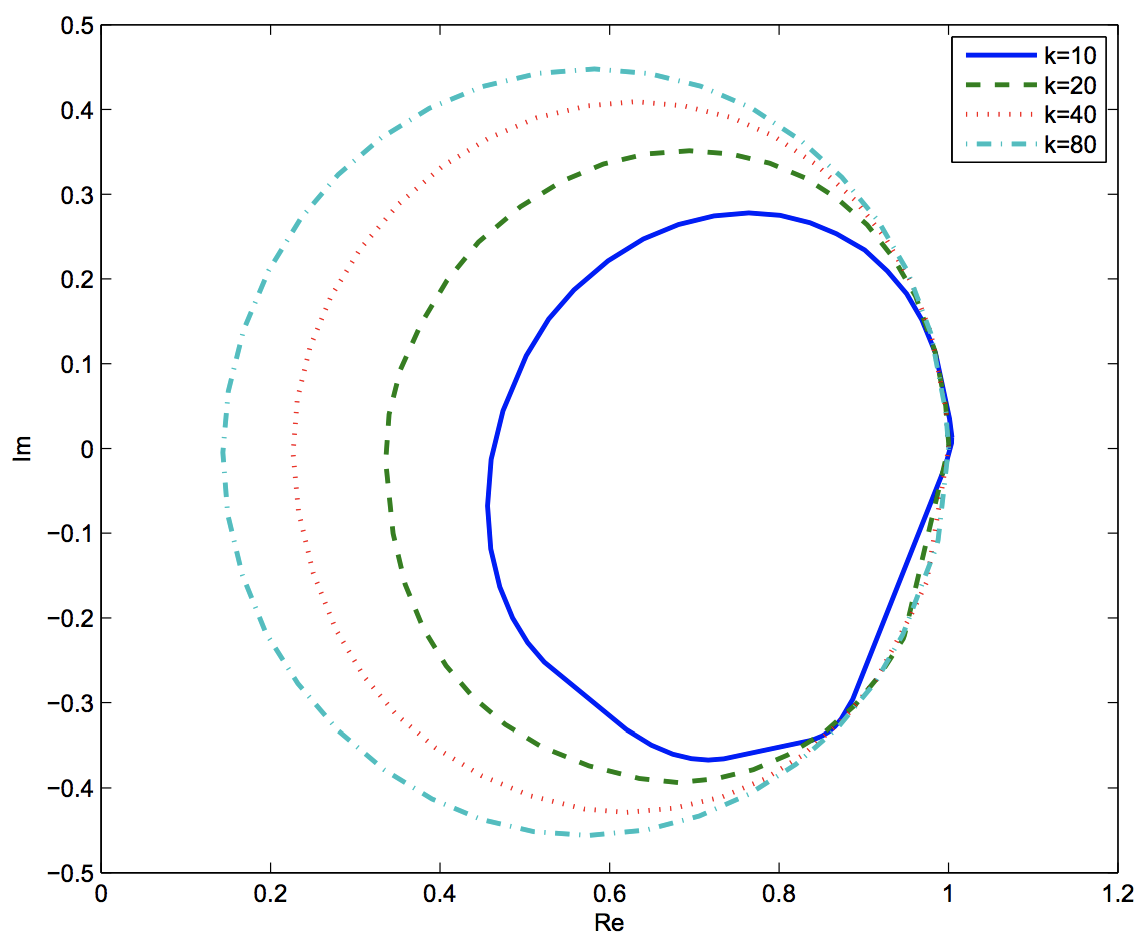
\includegraphics[width=.31\textwidth]{./Ref-fig/epsk32}}&
  {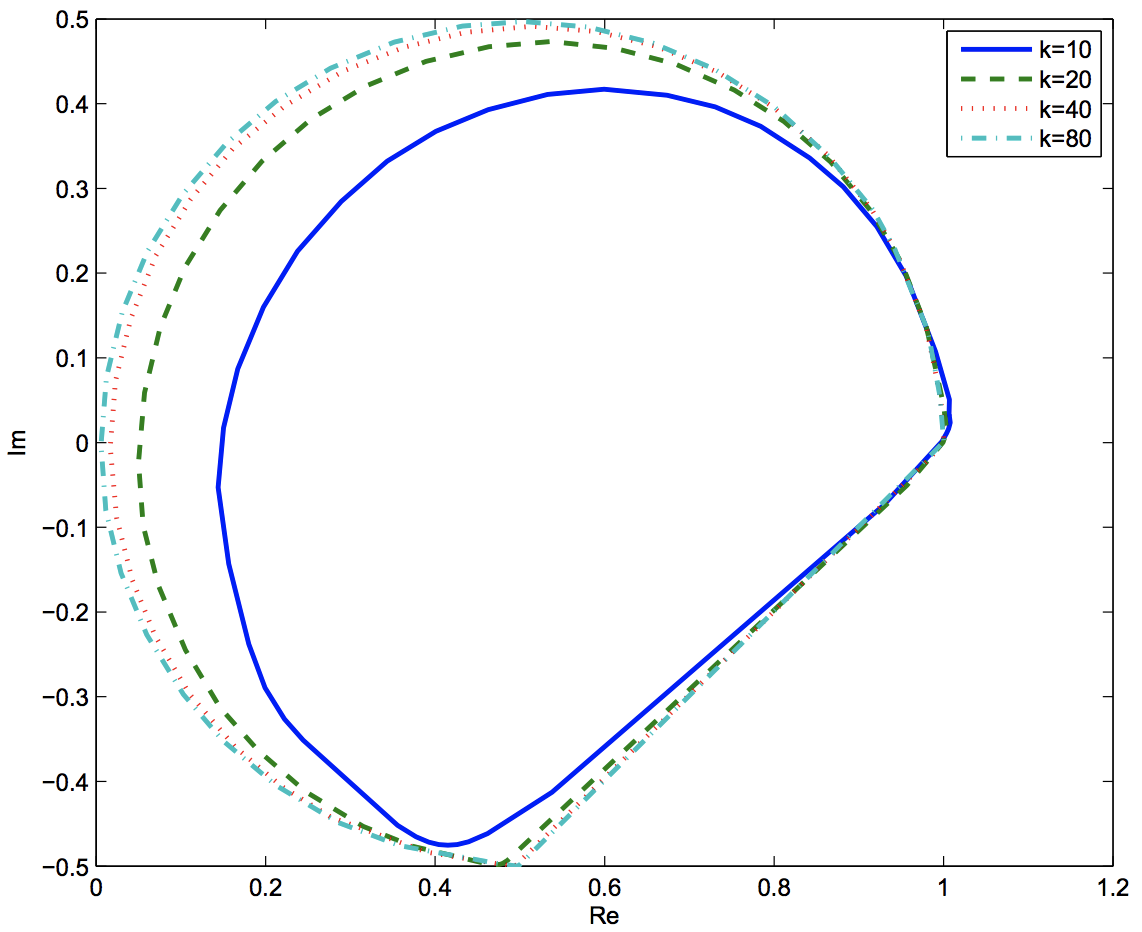
\includegraphics[width=.31\textwidth]{./Ref-fig/eps2}}
  \\
  (a) & (b) & (c)
\end{tabular}
\caption{Numerical range of $\mathbb{A}_{\epsilon}^{-1}\mathbb{A}$ for (a) $\epsilon=k$; (b) $\epsilon=k^{3/2}$; (c) $\epsilon = k^2$.}\label{fig:ex_ref}
\end{figure}

Figure \ref{fig:ex_ref} shows that when $\epsilon = k$, the numerical range remains bounded away from the origin as $k$ increases, whereas when $\epsilon = k^{3/2}$ or $\epsilon=k^2$ the distance of the numerical range from the origin decreases as $k$ increases.

% 1D results
\section{1-dimensional numerical experiment}
\subsection{Example 1} Let exact solution be $u=\sin(k\pi x)$.



\begin{thebibliography}{99}
\bibitem{Dolean2010}
V. Dolean, H. Fahs, L. Fezoui, and S. Lanteri. Locally implicit discontinous Galerkin method for time domain electromagnetics, J. Comput. Phys., 229 (2010): 512-526.

\bibitem{GuoCheng2016}
W. Guo and Y. Cheng. A Sparse Grid Discontinuous Galerkin Method for High-Dimensional Transport Equations and Its Application to Kinetic Simulations. SIAM J. Sci. Comput., 38(6), A3381-A3409. 

\bibitem{HoustonPerugiaSchneebeli2005b}
P. Houston, I. Perugia, A. Schneebeli, and D. Sch\"{o}tzau. Interior penalty method for the indefinite time-harmonic
Maxwell equations. Numer. Math., 100 (2005): 485-518.

\bibitem{Kopriva2002}
D.A.Kopriva, S.L.Woodruff and M.Y.Hussaini. Computation of electromagnetic scattering with a non-conforming discontinuous spectral element method, Int. J. Numr. Meth. Engng, 53 (2002): 105-122.

\bibitem{LiHesthaven2014}
J. Li and J.S.Hesthaven. Analysis and application of the nodal discontinuous Galerkin method for wave propagation in metamaterials, J. Comput. Phys., 258 (2014): 915-930.

\bibitem{ShuOsher1988}
C.W. Shu and S. Osher. Efficient implementation of essentially non-oscillatory shock-capturing schemes. J. Comput.
Phys., 77 (1988):439-471.


\bibitem{Warburton2000}
T. Warburton. Application of the discontinuous Galerkin method to Maxwell's equations using unstructured polymorphic hp-dinite elements, In Discontinuous Galerkin Methods, 2000, 451-458.

\bibitem{XieWangZhang2013}
Z. Xie, B. Wang and Z. Zhang. Space-Time discontinuous Galerkin method for Maxwell's equations, Commun. Comput.Phys., 14 (2013): 916-939.



\end{thebibliography}

\end{document}


